\subsection{Deep CVT Network}
\label{network}
This subsection describes the details of the Deep CVT Network, including its architecture, implementation, and training.

\begin{figure}[h]		
	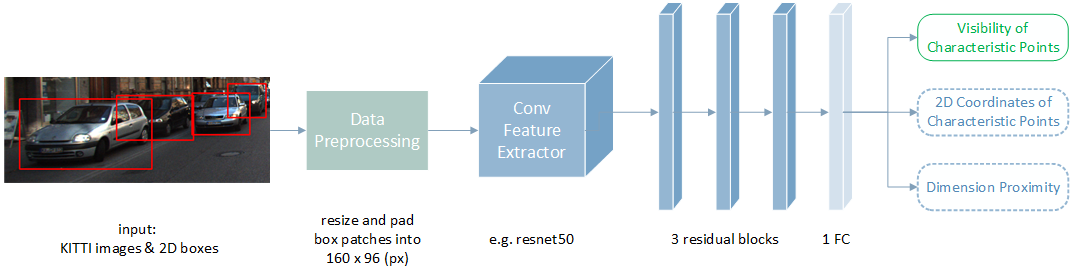
\includegraphics[width=1\textwidth]{NN_archi_box_0522.png}
	\caption{The Architecture of Deep CVT Network}
	\centering
	\label{figure:nn_archi}
\end{figure}

\subsubsection{Architecture}
The neural network is to learn a map from an N-dimensional  input space to an M-dimension output space. The map consists of several stages, called layers of the network, written as
\begin{equation}
Y = l_L(...l_2(l_1(X))), where ~Y \in {\mathbb{R}^M}, ~X \in {\mathbb{R}^N}
\end{equation}

Even through there are various layers, most layers  is composed of neurons, the basic computation element and most neurons are realized by linear and non-linear operations as 
\begin{equation}
a_{ij} = \sigma(W_{ij}^T X_i +b_j)
\end{equation}

where $a_{ij}$ is the result of the $i_th$ neuron in the $j_th$ layer, $\sigma$ is the activation function and $W_ij$ and $b_j$ are the weights vector and bias applied to input vector $X_i$.  The pooling layer is a special case which performs downsampling operations, such as max pooling \cite{Boureau:2010} and average pooling \cite{6460871}.

As shown in Figure \ref{figure:nn_archi}, our network follows the standard CNN architecture established in LeNet-5 \cite{726791}. It stacks a set of convolutional layers and pooling layers as a feature extractor, \tbd one fully-connected layers followed, and three output layers in the end. The goal of this network is to learn the 2D coordinates and visibility property of 20 interest points and the template proximity of the vehicle, given the RGB images captured by a monocular camera.

\paragraph{Input Layer}
The input layer accepts the input RGB images and feeds them into the network. In theory, images with arbitrary size can be accepted, but to make it more efficient, we use images with fixed resolution (96 x 160).  In this way, multiple images can be processed in one batch in order to reduce the variance of parameter updates and make the best use of highly optimized matrix optimizations during training \cite{DBLP:journals/corr/Ruder16}.

Since our approach is based on 2D object detection, each image contains at least one whole vehicle . To obtain these images, we first crop the patches defined by the 2D bounding box, then resize them to match one predefined dimension (96 or 160), and finally put the resized images in the center of the 96 x 160 canvas and padded with zeros for other pixel positions. We choose 96 x 160 as the fixed size because they are the means of sizes of all original patches so that we don't have to rescale the patch too much.  Some examples are shown in Figure \ref{figure:patches}.

\begin{figure}[h]		
	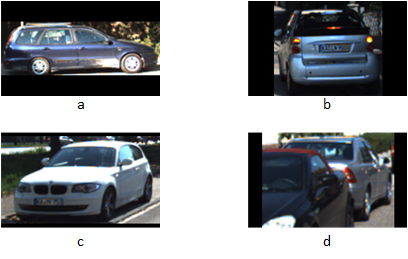
\includegraphics{patches.png}
	\caption{Examples of input images: a. the side view, b. the back view, c. the front view, d. the occluded case}
	\centering
	\label{figure:patches}
\end{figure}

\paragraph{Hidden Layers}
The hidden layers in out network consist of a feature extractor, 3 residual blocks \cite{DBLP:journals/corr/HeZRS15}, and a fully-connected layer. Both the feature extractor and residual blocks are composed of convolutional layers and pooling layers.

The feature extractor is actually one of available neural network models built in the Keras library \cite{chollet2015keras}, \ie VGG16, VGG19, Xception, ResNet50, \etc It is trained to  learn deep distributed hierarchical nonlinear representations of the input images.

 ResNet50 \cite{DBLP:journals/corr/HeZRS15} is chosen to be the benchmark model because it can ease the training and accelerate the convergence, especially for the fine tuning. It is well known that there are two main obstacles that hamper the training of deep neural networks: the vanishing/exploding gradient problem \cite{Bengio:1994:LLD:2325857.2328340, pmlr-v9-glorot10a} and the degradation problem that as the network is built deeper, the accuracy gets saturated or even degrades sharply \cite{DBLP:journals/corr/He014}. Residual nets are designed to address these two problems. Instead of learning the direct mapping from input to output, it learns a residual mapping first and then add the input to it, which just as Figure \ref{figure:residual_blocks} (a) shows. The paper validates that it is easier to learn the residual mapping than the direct one and the gradient can always pass through along the shortcut connections. Figure \ref{figure:residual_blocks} (b) and (c) shows two building blocks in our network. (b) is an identity block where the dimensions of input and output matches, while (c) is a linear projection block where the right branch performs $1\times1$ convolution to match the dimensions because the final addition is performed element-wisely.

\begin{figure}[h]		
	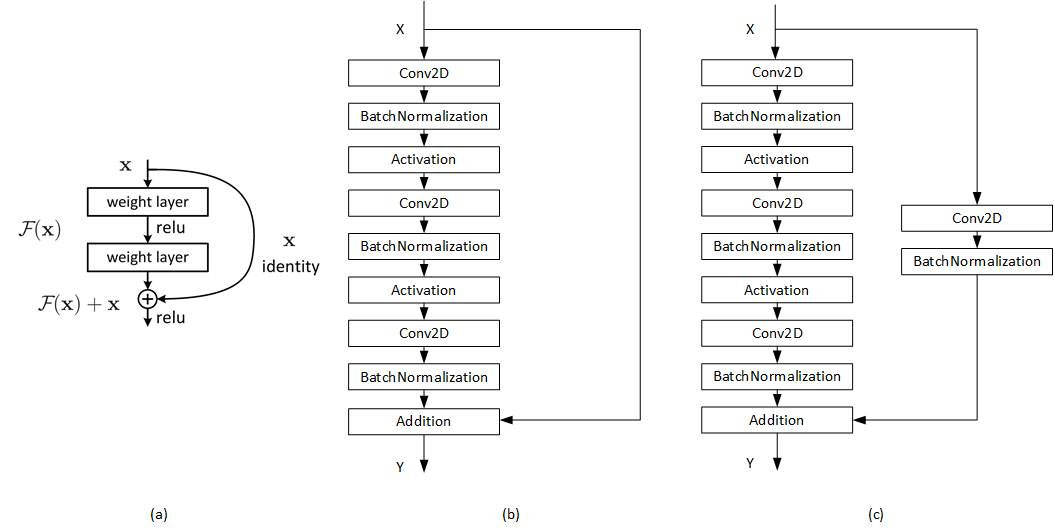
\includegraphics[width=1\textwidth]{residual_blocks.png}
	\caption{(a). a residual block \cite{DBLP:journals/corr/HeZRS15}, (b). an identity residual block in our network, (c). a linear projection residual block in our network}
	\centering
	\label{figure:residual_blocks}
\end{figure}

The last three residual blocks and a fully-connected layer is designed to learn non-linear combinations of the extracted features and then forward them to the output layers.

For all hidden layers, we all apply ReLU as the activation function. The function is

\begin{equation}
\label{relu}
f(z) = \max \{0, z\} ~~~~where~ z = W^TX+b
\end{equation}
This is a piecewise linear function consisting of two linear pieces, which makes the gradients through a rectified linear unit stay large and consistent whenever the unit is active. Papers \cite{pmlr-v15-glorot11a, Nair:2010:RLU:3104322.3104425, DBLP:journals/corr/JarrettKGL16} have validated that networks activated by ReLU can achieve much better performance than others. ReLU preserves many properties that make the model easy to optimize with gradient-based methods and generalize well, while introducing non-linearity into the model \cite{Goodfellow-et-al-2016}. 

\paragraph{Output Layers}
\label{output}

Our network has three kinds of output layer for the three tasks respectively. For 2D coordinates regression, a 40-neuron layer with linear activation function is provided.  Each neuron's output indicates one coordinate value, \ie $x_i$ or $y_i$.  20 coordinates are arranged in an ascending order. For visibility characterization, we implement 20 independent quaternary classifiers for 20 points. Each classifier is associated with a softmax activation function \cite{Bishop:2006:PRM:1162264} which outputs four values representing the probabilities of each target class over all possible classes. Template proximity is equipped with a 154-neuron linear layer for regression.  Each neuron indicates one ratio element of the template proximity vector. Eq.\ref{linear} is a linear activation function while Eq.\ref{softmax} is a softmax activation function.

\begin{equation}
\label{linear}
out_i = W_i^TX_i+b_i
\end{equation}

\begin{equation}
\label{softmax}
out_i = \frac{e^{W_i^TX_i+b_i}}{\sum_{k=1}^K e^{W_k^TX_k+b_k}}
\end{equation}


\subsubsection{Training}

\paragraph{Multi-task Learning}
As mentioned in Section \ref{output}, our network has totally 22 output layers. This implementation makes use of multi-task learning (MTL) where multiple learning tasks are trained parallel based on the shared features. Caruana has validated that tasks trained in MTL have better generalization performance than trained in a single-task learning mode \cite{Caruana1997}. And he summarizes that this improvement results from leveraging the domain-specific information contained in the training signals of other related tasks \cite{Caruana1997}. Therefore, we follow this paradigm to design our network in order to achieve better performance.

\paragraph{Loss Functions}
The learning of 2D coordinates and template proximity are regression tasks so that a robust smooth $L_1$ loss function \cite{DBLP:journals/corr/Girshick15} is chosen for them. We modify it as
\begin{equation}
\label{eq10}
smooth_{L_1}(x) =
\begin{cases}
~0.5x^2 ~~~~~~~~~~~~if ~\left | x \right |< 0.5 & \\    
~\left | x \right | -0.25 ~~~~~otherwise   
\end{cases} 
where  ~ x=\widehat{y} - y
\end{equation}
Compared to $L_2$ loss, it is less sensitive to outliers and no special attention is required to pay in order to prevent gradient exploding problem\cite{DBLP:journals/corr/Girshick15}. Besides, when applied with gradient-based optimization, $L_1$ loss and $L_2$ loss often result in poor performance \cite{Goodfellow-et-al-2016}.

For visibility characterization, we develop a model for probabilistic classification so that categorical cross-entropy is used as the loss function. It is also known as the negative log-likelihood \cite{Goodfellow-et-al-2016}, defined as:

\begin{equation}
\label{eq11}
L_{cce} =\frac{1}{N} \sum_{n=1}^N H(y,\widehat{y}) = -\frac{1}{N}\sum_{n=1}^N \sum_{i=1}^c y_{n,i} \log \widehat{y}_{n,i}
\end{equation}

where $H(y, \widehat{y})$ denotes the cross-entropy between the ground truth probability distribution $y$ and the predicted $\widehat{y}$, and $y_{n,i} $ represents the true probability of $i_{th}$ class for the $n_{th}$ data example $\widehat{y}_{n,i}$ is the estimated. It is a continuous convex loss function which measures the discrepancy between the true and estimated distributions multi-class classification tasks \cite{DBLP:journals/corr/abs-1802-09941} which means it can measure the degree of correctness, \ie it can distinguish between "nearly correct" and "totally wrong" cases.  Therefore, it outperforms other loss functions in classification tasks and then becomes ubiquitous in deep learning nowadays.


\paragraph{Normalization}
Normalization is an important pre-processing step in deep learning which ensures that each feature has a similar data distribution. This is usually done by restricting the features in certain range or standardizing their ranges. It can enhance the learning capability of the network and speed up the convergence substantially  because it can reduce the bias among features and decrease the low and high frequency noisy in data \cite{Jayalakshmi2011}. The speed-up mechanism can be concluded from Figure \ref{figure:contour}. If we initialize the network at point A in Figure \ref{figure:contour} (a), the gradient-descent update routine will oscillate along the long axis of the eclipse, which definitely takes more time to reach the optimum than any arbitrary initial point in Figure \ref{figure:contour} (b) where the update trajectory is almost a straight line for any starting point  to the minimum. Besides, this also helps the performance because the update trajectory oscillates less around the minimum for case (b) than case (a) so that it is more possible for case (b) to reach the optimum.

\begin{figure}[h]		
	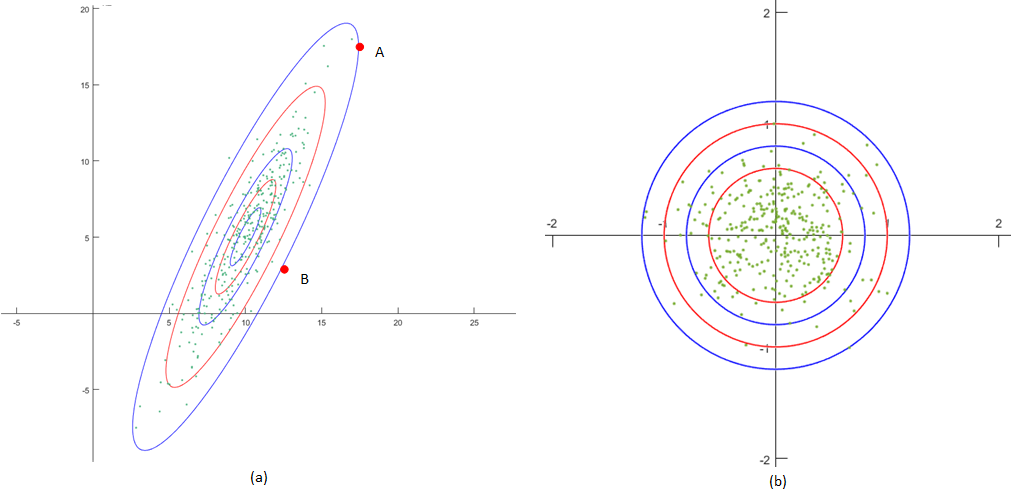
\includegraphics[width=1\textwidth]{contour.png}
	\caption{(a). data distribution before normalization, (b). data distribution after normalization}
	\centering
	\label{figure:contour}
\end{figure}

Our network takes RGB images as input so that pixel intensity is the input feature. The technique we use to normalize the image is channel mean subtraction, used in \cite{DBLP:journals/corr/SimonyanZ14a, DBLP:journals/corr/GirshickDDM13}, which centers all the features around the origin along each dimension.As mentioned in CS231N \cite{CS231N}, mean channel subtraction is enough for CNNs and the original range of pixel values is determined, \ie $[0, 255]$.

The range of ground truth influences the loss. In order to make the three labels impact similarly on the loss, we normalize them. For visibility, we use one-hot-encoding \cite{One-hot} to encode its classes so that it only has value 0 or 1. The value of 2D coordinates $C^{2d}  = \{p_1, p_2, ...,p_{20}\}$varies a lot so that we normalize them w.r.t. the associated 2D bounding box $B^{2d} = (c_u, c_v, w, h)$ \cite{DBLP:journals/corr/ChabotCRTC17}. The normalized 2D coordinates $\overline{C}^{2d}  = \{\overline{p}_1, \overline{p}_2, ...,\overline{p}_{20}\}$ ranges $[-1, 1]$, where
\begin{equation}
\overline{p}_i  = (\frac{u_i - c_u}{w}, \frac{v_i - c_v}{h})
\end{equation}

The template proximity vector $T$  is normalized with $\log$ function element-wisely \cite{DBLP:journals/corr/ChabotCRTC17}, resulting in $\overline T$ so that the range falls into $[-1, 1]$, too.

Moreover, as Sergey \etal \cite{DBLP:journals/corr/IoffeS15}states the variation of each layer's input distribution during the training makes the training complicated and hard to converge quickly so that we apply Batch Normalization (BN) to alleviate the internal covariate shift phenomenon.  BN normalizes the summed activations of each layer to a distribution of zero mean and unit variance. The mean and variance of each activation is computed on each mini-batch. By doing so, much larger learning rate can be used for training and no special attention has to pay on parameter initialization. 
 
\paragraph{Regularization}
Regularization techniques are used to address the overfitting problem in order to make an algorithm not only perform well on the training data but also on the test data, the previously unseen data \cite{Goodfellow-et-al-2016}. Overfitting results from either that the algorithm is too complicated for the data or that the sampled data is not able to represent the internal pattern. Normally, we design an algorithm to model  the data pattern exhaustively first and then apply regularization techniques to make the algorithm generalize well.  

In the data aspect, we use data augmentation as a regularization. The best way to address overfitting is to train the model on more data, while the amount of data is restricted for one dataset. Therefore we generate some synthetic data. Since our network involves with classification and regression tasks, we mainly enlarge the dataset via flipping, scaling, and cropping \tbd. 

In the architecture aspect, Batch Normalization \cite{DBLP:journals/corr/IoffeS15} is used as the regularization in each layer. BN enables the network to obtain the information of the training sample and the others in mini-batch simultaneously so that it does not generate deterministic dependency on this training sample. Therefore BN can replace Dropout \cite{JMLR:v15:srivastava14a} to be the regularization for our convolutional network. 

Besides, Multitask Learning is another technique we used to improve generalization performance. 
In our network, the learning representation is shared across all tasks so that the parameters shared are constrained to bias towards one specific task, \ie only the representation that is useful for more than one can be kept \cite{Goodfellow-et-al-2016}.  Therefore statistical strength of the parameters is highly enhanced \cite{Baxter:1995:LIR:225298.225336}.

During the training, early stopping is applied to prevent the model being trained too complex to fit the test data. As Figure \ref{figure:early_stopping} shows, we halt the training when the validation error stops decreasing.  The stopping point is when the learned model can represent the pattern of validation data most. It regards the number of training epochs as a hyperparameter and can effectively tune it to be optimal \cite{DBLP:journals/corr/abs-1206-5533},  because early stopping can restrict the global learning capacity of a large network to fit simpler dataset without affecting the backpropagation to control the learning capacity locally \cite{Caruana:2000:ONN:3008751.3008807}.


\begin{figure}[h]		
	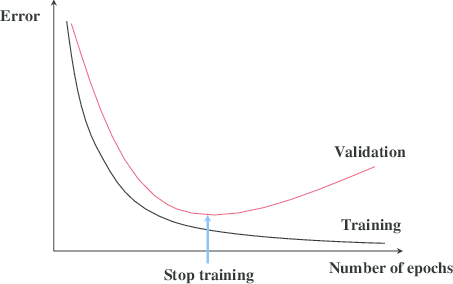
\includegraphics{early_stopping.png}
	\caption{Early stopping}
	\centering
	\label{figure:early_stopping}
\end{figure}

\paragraph{Parameter Initialization}

Transfer learning is proposed to transfer the representation learned from one task to another related task \cite{Pan:2010:STL:1850483.1850545}. As is known that CNNs learn more abstract features in a deeper layer. It is not surprising to find that, for visual tasks, shallow layers learn low-level features, \eg edges, corners, changes in lighting, \etc, which are shared across datasets and tasks. Moreover, Yosinski \etal validate \cite{DBLP:journals/corr/YosinskiCBL14} that initializing a network with transferred features can improve the generalization capability hugely and Yoshua \etal \cite{NIPS2006_3048} confirm that this initialization put the start point closer to a local minimum than random initializations, resulting in accelerating convergence.

Therefore we initialize our feature extractor with parameters learned on ImageNet dataset \cite{DBLP:Russakovsky14} and the three residual blocks with parameters trained on the KITTI dataset. The fully-connected layer is initialized from a zero-mean Gaussian distribution with standard deviation 0.01 and all the output layers are initialized with zeros.


\paragraph{Learning Algorithms / Optimization}

Optimization is a task of finding the value $x$ in order to minimize or maximize some objective function $f(x)$. One most powerful optimization technique category in deep learning is gradient-based.

As is known, the derivative $f'(x)=\frac{\text{d}y}{\text{d}x}$ specifies how to make a small change $\epsilon$ of the input $x$ to get the corresponding change in the function:
\begin{equation}
	f(x + \epsilon)~ \approx ~ f(x) + \epsilon f'(x).
\end{equation}

Thus, the derivative tells the direction to minimize a function, i.e. it can point out how to change $x$ to make a small update. One popular algorithm, gradient descent \cite{gd1847}, makes use of the derivatives and update the input $x$ directly as:

\begin{equation}
x = x - \alpha {\triangledown} _x f(x)
\end{equation}

where $\alpha$ is the learning rate, a positive real value to decide the size of an update step. The examples in Figure \ref{figure:optimization} (a) show how the update works.  A deep network often consists of many layers so that back-propagation algorithm \cite{Rumelhart:1988:LRB:65669.104451} is used to compute the gradient for each parameter in different layers of the objective function based on the chain rule of calculus.

\begin{figure}[h]		
	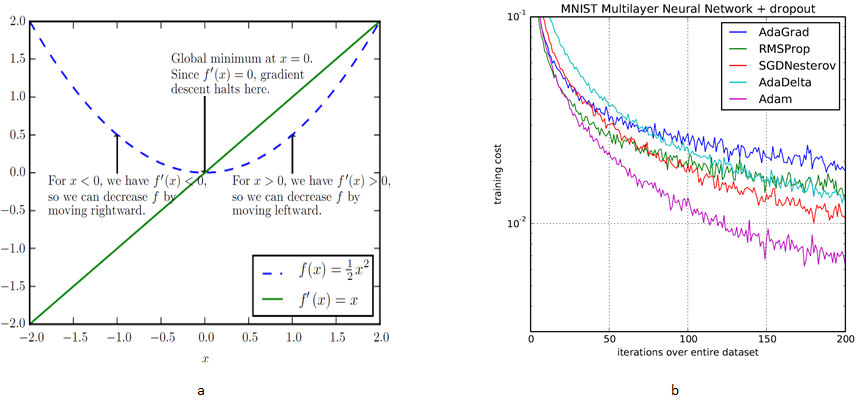
\includegraphics[width=1\textwidth]{optimization.png}
	\caption{(a). examples to show how gradient decent makes use of derivatives to reach a minimum \cite{Goodfellow-et-al-2016}, (b). performance of optimization algorithms in the same setting \cite{DBLP:journals/corr/KingmaB14}}
	\centering
	\label{figure:optimization}
\end{figure}

In deep learning, the input to the objective function is often multidimensional so that it probably has many local minima and saddle points, which renders huge difficulties to optimization. Therefore we usually take in a compromise scenario where the value $x$ makes $f$ really low but not necessarily globally minimal \cite{Goodfellow-et-al-2016}.

The optimization algorithm we used is Adam \cite{DBLP:journals/corr/KingmaB14} which is robust and efficient in memory and computation for the optimization of stochastic objectives with high-dimensional parameters spaces. It makes use of both the gradient and its momentum to update parameters as: 

\begin{algorithm}[H]	
	\While{$x_t$ not converged}{
		$ t = t + 1 $\;
		$ g_t = {\triangledown} _x f(x_{t-1}) $\;
		$ m_t = \beta_1 m_{t-1} + (1-\beta _1) g_t$ \;
		$ v_t = \beta_2 v_{t-1} + (1-\beta_2) g_t^2 $\;
		$ \hat{m}_t = \frac{m_t}{1 - \beta _1^t} $\;
		$ \hat{v}_t = \frac{v_t}{1 - \beta_2^t}  $\;
		$ x_t = x_{t-1} - \alpha \frac{\hat{m}_t}{\sqrt{\hat{v}_t} + \epsilon}$\;
	}
	%\caption{Adam algorithm update mechanism}
\end{algorithm}

where $ t $ denotes the current iteration, $\alpha$ is the learning rate, $\beta_1$ and $\beta_2$ are two exponential decay rates, and $\epsilon$ is a small scalar to prevent zero-division.

From the Figure \ref{figure:optimization} (b), we can see that Adam can make the learning task converge relatively faster and has lower training error so that we follow this guide to apply Adam in our optimization of CVT Network.
